\documentclass[aspectratio=169]{beamer}
%\documentclass[xcolor=pst,dvips,epic,eepic]{beamer}

\usepackage[utf8]{inputenc}
\usetheme{Singapore}
\usepackage{xcolor}
\setbeamertemplate{footline}[frame number]

\usepackage{../sty/mathlist}

\usepackage{amsmath,amssymb, amsthm}
\usepackage{amscd}

%\newtheorem{theo}{Théorème}

\usepackage{pstricks, pst-node}

\usepackage{tikz}
\usetikzlibrary{arrows,positioning}

\usepackage{times}

\usepackage{ulem}

\usepackage{listings}
%\topmargin=-0.6in
\lstloadlanguages{C++}
\lstset{language=C++}
%%}

\setbeamercovered{dynamic}

\input{../sty/macros}

\def\bxi{\boldsymbol\xi}
\def\bomega{\boldsymbol\omega}
\def\bC{\boldsymbol{C}}
\def\bu{\boldsymbol{u}}
\def\bU{\boldsymbol{U}}
\def\by{\boldsymbol{y}}
\def\vol{\mbox{vol}}

\def\blue{\color{blue}}
\def\red{\color{red}}

\title[Random Numbers Generation]{A short tutorial on random number generation}

\author[Fabian Bastin]{Fabian Bastin \\ \url{fabian.bastin@umontreal.ca} \\ Université de Montréal -- CIRRELT -- IVADO}
\date{}

\begin{document}
	
\titlegraphic{\vspace{-0.5cm}
	
\includegraphics[scale=0.2]{udem.png}
}
	\frame{\titlepage}
	

\begin{frame}
	%\frametitle{Outline}
	%

\begin{center}
	\href{https://xkcd.com/221/}{
\includegraphics[scale=0.75]{random_number.png}}
\begin{small}
	\url{https://xkcd.com/221/}
\end{small}
\end{center}

%\begin{center}

%	\href{https://xkcd.com/221/}{
\includegraphics[scale=0.75]{imgs/random_number.png}}
%	\begin{small}
%		\url{https://xkcd.com/221/}
%	\end{small}

%\end{center}

\end{frame}
	
	\begin{frame}
		\frametitle{U[0,1]-distributed random numbers}
		
		\begin{itemize}
			\item
			A good uniform random generator on the interval $[0,1]$ is a major
			component of any good random generator library.
			\item
			Draws from other distributions are usually obtained by adequately transforming a
			uniformly distributed sample.
		\end{itemize}
		
		\mbox{}
		
		Define a {\blue transition function} $f: \mathcal{S} \rightarrow \mathcal{S}$,
		where $\mathcal{S}$ is the {\blue state space}.
		The cardinality of $\mathcal{S}$ is assumed to be finite.
		
		\mbox{}
		
		The initial state is denoted by $s_0$, and we will write
		\[
		s_n = f(s_{n-1}).
		\]
		We will furthermore assume that $f$ is periodic for all $n$ greater than
		or equal to some known $\tau$ (often equal to 0), with period $\rho$:
		$$
		s_{n+\rho} = s_n,\ \forall\, n\ge\tau.
		$$
		
	\end{frame}
	
	\begin{frame}
		\frametitle{U[0,1]-distributed random numbers (cont'd)}
		
		\begin{itemize}
			\item
			Output space: $\mathcal{U}$.
			\item
			We assume here that $\mathcal{U} = (0,1)$.
			\item
			Output function $g: \mathcal{S} \rightarrow \mathcal{U}$.\\
			It transforms the state $s_n$ into an output value $u_n$.
		\end{itemize}
		
		\begin{small}
			\[
			\begin{CD}
				\cdots @>f>> s_{\rho-1} @>f>> s_0 @>f>> s_1  @>f>> 
				\cdots @>f>> s_n @>f>> \cdots \\ 
				%
				@. @V{g}VV  @V{g}VV   @V{g}VV   
				@.  @V{g}VV  \\
				%
				\cdots @. u_{\rho-1} @. u_0
				@.  u_1  @.   \cdots @.  u_n @.  \cdots \\
			\end{CD}
			\]
			\label{fig:rng}
		\end{small}
		
		\mbox{}
		
		{\bf How to choose $f$ and $g$?}
		
		\mbox{}
		
		\textcolor{red}{Goals:} large $\rho$, good uniformity, ``random'' behavior.
		
	\end{frame}
	
	\begin{frame}
		\frametitle{Linear congruential generators (LCGs)}
		
\begin{itemize}
\item
Introduced by Lehmer (1951).
\item
State $s = x \in \NN_{\geq 0}$.
\item
Recursive formula:
$$
x_i = f(x_{i-1}) = (ax_{i-1}+c) \mod m,
$$
where $\mod$ is the modulo operator: given a dividend $p$ and a divisor
$q > 0$,
$$
p \mod q = p - q\left\lfloor \frac{p}{q} \right\rfloor.
$$
\item
If $c = 0$, the generator is often called a multiplicative congruential generator, or ``{\red Lehmer RNG}''
\end{itemize}
		
\end{frame}
	
	\begin{frame}
		\frametitle{Linear congruential generators: full period?}
		
		Full period: $m$ if $c \ne 0$, $m-1$ otherwise (if $c = 0$, 0 is a
		fixed point for the recurrence).
		Consider the case $c \ne 0$.
		
		\begin{theorem}[Period]
			The LCG has full period iff the
			following three conditions hold:
			\begin{enumerate}
				\item
				the only positive integer that (exactly) divides both $m$ and $c$ is
				1;
				\item
				if $q$ is a prime number that divides $m$, then $q$ divides $a-1$;
				\item
				if 4 divides $m$, then 4 divides $a-1$.
			\end{enumerate}
		\end{theorem}
		``{\red Standard minimal}'' (Park and Miller, 1988):
		\[
		x_{n+1} = 16807x_n \mbox{ mod } 2147483647.
		\]
		Observe that $2147483647 = 2^{31}-1$; on 32-bit architectures, the
		largest representable (signed) integer is $2^{31}-1$.
		
	\end{frame}
	
	\begin{frame}[containsverbatim]
		\frametitle{The Standard Minimal Generator}
		
		\begin{small}
			\begin{verbatim}
function getlcg(seed::Integer, a::Integer,
                 c::Integer, m::Integer)
    state = seed
    am_mil = 1.0/m
    return function lcgrand()
        state = mod(a * state + c, m)
        # produce a number in (0,1)
        return state*am_mil
    end
end

stdmin = getlcg(1234, 16807, 0, 2^31-1)
		\end{verbatim}
		\end{small}
		
	\end{frame}
	
	\begin{frame}
		\frametitle{Standard minimal generator: illustration}
		\begin{center}
			
\includegraphics[width=0.65\linewidth]{lcg.png}
			
			10000 generated points on the unit square.
		\end{center}
		
	\end{frame}
	
	\begin{frame}
		\frametitle{Multiple Recursive Generator (MRG)}
		
		But we want better! Generalize the LCG:
		\[
		x_n = (a_1 x_{n-1} + \cdots + a_k x_{n-k}) \mod {m}, \quad  
		u_n = x_n / m.
		\]
		In practice, take $u_n = (x_n + 1) / (m+1)$, or $u_n =
		x_n/(m+1)$ if $x_n>0$ and $u_n = m/(m+1)$ otherwise, but the structure
		remains the same, and is easier when studying theoretical properties.
%		This kind of generators is very popular.
		
		\mbox{}
		
		State at step $n$:
		\[
		s_n = (x_{n-k+1},\dots,x_n)^T.
		\]
		State space: $\ZZ_m^k$, of cardinality $m^k$.
		
		\mbox{}
		
		The maximal period is $\rho = m^k-1$.
		
	\end{frame}
	
	\begin{frame}
		\frametitle{Period of MRGs}
		
		It can be shown that, for $k > 1$, the maximal period can already be
		reached with only {\blue two} non-zero coefficients, including $a_k$ ---
		provided they are suitably chosen.
		
		\mbox{}
		
		The cheapest recurrence has therefore the form
		\[
		x_n = (a_r x_{n-r} + a_k x_{n-k}) \mod m.
		\]
		
		\mbox{}
		
		But how to choose $a_r$ and $a_k$?
		
		\mbox{}
		
		It is possible to study theoretical properties of MRG's, and exclude
		directly some generators that have known strong deficiencies.
		
	\end{frame}
	
	\begin{frame}
		\frametitle{Choosing a good MRG}
		
		{\blue Example: Lagged-Fibonacci}
		\[
		x_n = (\pm x_{n-r} \pm x_{n-k}) \mod m.
		\]
		It can be shown that the vectors $(u_n, u_{n+k-r}, u_{n+k})$ are all
		contained in two planes! We therefore know without additional tests
		that the numbers cannot be considered as random.
		
		\mbox{}
		
		In practice, we can impose various conditions on the coefficients, and
		compute theoretically appealing generators by maximizing some quality
		measure. This maximization is numerically expensive.
		
	\end{frame}
	
	\begin{frame}
		\frametitle{Combined MRG's}
		
		Consider two (or more) MRG's working in parallel:
		\begin{eqnarray*}
			x_{1,n} &=& (a_{1,1} x_{1,n-1} + \cdots + a_{1,k} x_{1,n-k}) \mod m_1,\\
			x_{2,n} &=& (a_{2,1} x_{2,n-1} + \cdots + a_{2,k} x_{2,n-k}) \mod m_2.
		\end{eqnarray*}
		We define the two {\red combinations}
		$$
		\begin {array}{rclrcl}
		z_n &:=& (x_{1,n} - x_{2,n}) \mod m_1; &
		{u_n} &:=& z_n/m_1; \\
		{w_n} &:=& (x_{1,n}/m_1 - x_{2,n}/m_2) \mod 1.
		\end {array}
		$$
		
		\mbox{}
		
		The sequence ${\{w_n,\, n\ge 0\}}$ is the output of another MRG, of
		modulus ${m} = m_1 m_2$, and ${\{u_n,\, n\ge 0\}}$ is nearly the same
		sequence if $m_1$ and $m_2$ are close.\\
		We can achieve the period $(m_1^k-1)(m_2^k-1)/2$.
		
	\end{frame}
	
	\begin{frame}
		\frametitle{MRG32k3a}
		
		The following combined MRG was proposed by L'Ecuyer. It has been for a long time
		amongst the most popular and efficient generators (e.g., used in R), although newer
		families like xoshiro or CBRNGs are often preferred today for raw performance.
		It combines 2 MRG's.
		
		$k=3$, \\
		$m_1 = 2^{32} -209$, $a_{11} = 0$, $a_{12} = 1403580$, $a_{13} = -810728$,\\
		$m_2 = 2^{32}-22853$, $a_{21} = 527612$, $a_{22} = 0$, $a_{23} = -1370589$.\\
		
		\mbox{}
		
		Combination: $z_n = (x_{1,n} - x_{2,n}) \bmod m_1$.
		
		\mbox{}
		
		Corresponding MRG: $k=3$,\\
		$m = m_1 m_2 = 18446645023178547541$, \\
		$a_{1} = 18169668471252892557$,\\
		$a_{2} = 3186860506199273833$,\\ 
		$a_{3} = 8738613264398222622$.
		
		\mbox{}
		
		Period $\rho = (m_1^3-1)(m_2^3-1)/2 \approx 2^{191}$.
	\end{frame}
	
	\begin{frame}[containsverbatim]
		\frametitle{MRG32k3a: basic implementation}
		
		\begin{footnotesize}
			\begin{verbatim}
function rand(rng::MRG32k3a)

p1::Int64 = (a12 * rng.Cg[2] + a13 * rng.Cg[1]) % m1
p1 += p1 < 0 ? m1 : 0

rng.Cg[1] = rng.Cg[2]
rng.Cg[2] = rng.Cg[3]
rng.Cg[3] = p1
p2::Int64 = (a21 * rng.Cg[6] + a23 * rng.Cg[4]) % m2
p2 += p2 < 0 ? m2 : 0

rng.Cg[4] = rng.Cg[5]
rng.Cg[5] = rng.Cg[6]
rng.Cg[6] = p2
u::Float64 = p1 > p2 ? (p1 - p2) * norm :
   (p1 + m1 - p2) * norm
end
			\end{verbatim}
			\end{footnotesize}
			
		\end{frame}

		
\begin{frame}
		\frametitle{Random numbers generators on $\FF_2$}
		
		MRGs work on integers. An alternative is to build generators directly
		on {\blue bits}, with {\blue linear recurrences in}\, $\FF_2$.
		
		\vspace{0.2cm}
		
		Let us introduce the Galois field $\FF_2$: it is simply the set $\lbrace 0,1 \rbrace$
		with addition and multiplication computed modulo 2.
		
		\vspace{0.2cm}
		\begin{columns}
		\begin{column}{0.45\textwidth}
		\centering
		\textbf{Addition} ($\oplus$, XOR) \\
		\vspace{0.1cm}
		\begin{tabular}{c|cc}
		$\oplus$ & 0 & 1 \\
		\hline
		0 & 0 & 1 \\
		1 & 1 & 0
		\end{tabular}
		\end{column}
		
		\begin{column}{0.45\textwidth}
		\centering
		\textbf{Multiplication} ($\cdot$, AND) \\
		\vspace{0.1cm}
		\begin{tabular}{c|cc}
		$\cdot$ & 0 & 1 \\
		\hline
		0 & 0 & 0 \\
		1 & 0 & 1
		\end{tabular}
		\end{column}
		\end{columns}
		
		\vspace{0.4cm}
		
		All operations are then {\blue bitwise} (shifts, xors, masks),
		which makes these generators {\blue numerically very fast}.
		
	\end{frame}
	
	\begin{frame}
		\frametitle{Generators on $\FF_2$: state and output}
		
		We construct two sequences of bit vectors, the {\blue state} and the
		{\blue output}, with linear recurrences ($k$-bit state, $w$-bit output):
		\begin{align*}
			\boldsymbol{x}_n &= {X} \boldsymbol{x}_{n-1} & \quad \mbox{(state vector, $k$ bits)},\\
			\boldsymbol{y}_n &= {B} \boldsymbol{x}_{n}  & \quad \mbox{(output vector, $w$ bits)},
		\end{align*}
		where $X$ and $B$ are binary matrices and all arithmetic is in $\FF_2$.
		
		\mbox{}
		
		{\blue Reading a binary fraction.} The $w$ output bits are stacked after the radix point:
		\[
			u_n = \sum_{j=1}^w y_{n,j-1}\, 2^{-j} = .y_{n,0}\; y_{n,1}\; \ldots\; y_{n,w-1}.
		\]
		Example: $y_n = (1,0,1,1)$ gives $2^{-1} + 2^{-3} + 2^{-4} = 0.6875 = .1011_2$.
		
	\end{frame}
	
	\begin{frame}
		\frametitle{LFSR: a shift register with linear feedback}
		
		\begin{minipage}{0.57\linewidth}
			A {\blue linear feedback shift register} (LFSR) is a $k$-bit register
			updated in three steps:
			\begin{enumerate}
				\item
				read the {\blue tapped bits} --- here the positions $r$ and $k$;
				\item
				{\blue xor} them: the new bit is $x_n = x_{n-r} \oplus x_{n-k}$
				(it is read before the shift);
				\item
				{\blue shift} the register by one position and insert $x_n$.
			\end{enumerate}
		\end{minipage}
		\hfill
		\begin{minipage}{0.40\linewidth}
			\begin{center}
			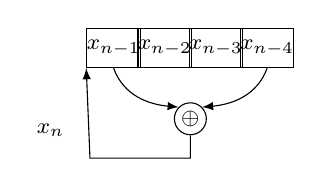
\begin{tikzpicture}[
				box/.style={draw, minimum width=0.55cm, minimum height=0.5cm, font=\footnotesize, inner sep=0pt},
				>=latex]
				\node[box] (b1) at (0,0)    {$x_{n-1}$};
				\node[box] (b2) at (0.65,0) {$x_{n-2}$};
				\node[box] (b3) at (1.3,0)  {$x_{n-3}$};
				\node[box] (b4) at (1.95,0) {$x_{n-4}$};
				\node[circle,draw,inner sep=1pt,font=\footnotesize] (xor) at (0.975,-0.9) {$\oplus$};
				\draw[->] (b1.south) to[out=-70,in=175] (xor.north west);
				\draw[->] (b4.south) to[out=-110,in=5]  (xor.north east);
				\draw[->] (xor.south) -- (0.975,-1.4) -- (-0.3,-1.4) -- (b1.south west);
				\node[font=\footnotesize] at (-0.8,-1.05) {$x_n$};
			\end{tikzpicture}
			\end{center}
		\end{minipage}
		
	\end{frame}
	
	\begin{frame}
		\frametitle{LFSR: a tiny example ($k = 4$, taps $r = 1$ and $k = 4$)}
		
		Seed $0001$, recurrence $x_n = x_{n-1} \oplus x_{n-4}$:
		\begin{center}
			\footnotesize
			\setlength{\tabcolsep}{4pt}
			\begin{tabular}{r|cccc|c}
				step & \multicolumn{4}{c|}{register} & new bit\\
				& $x_{n-1}$ & $x_{n-2}$ & $x_{n-3}$ & $x_{n-4}$ & $x_n$\\
				\hline
				0 & 0 & 0 & 0 & 1 & \text{--}\\
				1 & 1 & 0 & 0 & 0 & 1\\
				2 & 1 & 1 & 0 & 0 & 1\\
				3 & 1 & 1 & 1 & 0 & 1\\
				4 & 1 & 1 & 1 & 1 & 1\\
				$\vdots$ & & & & & \\
				7 & 0 & 1 & 0 & 1 & 0\\
				8 & 1 & 0 & 1 & 0 & 1\\
				9 & 1 & 1 & 0 & 1 & 1\\
				$\vdots$ & & & & & $\vdots$
			\end{tabular}
		\end{center}
		
		\begin{itemize}
			\item
			After $15$ steps we are back to the seed $0001$: period $2^4 - 1$.
			\item
			All $2^4-1$ {\blue non-zero} states have been visited: {\blue maximal period}.
		\end{itemize}
		
	\end{frame}
	
	\begin{frame}
		\frametitle{LFSR: matrix form}
		
		The recurrence is a linear recurrence over $\FF_2$ on the state vector
		(we assume $a_k \ne 0$):
		\[
			\boldsymbol{x}_n = X\, \boldsymbol{x}_{n-1},
			\qquad
			X =
			\begin{pmatrix}
				0    & 1      &        &        \\
				     & \ddots & \ddots &        \\
				     &        & \ddots & 1      \\
				a_k  & a_{k-1} & \ldots & a_1
			\end{pmatrix}.
		\]
		
		\begin{itemize}
			\item
			The {\blue last row} encodes the taps (the feedback coefficients), the rest of
			the matrix is a pure shift.
			\item
			$X^\nu$ shifts the register by $\nu$ bits in one step: this is the spacing
			$\nu$ used when assembling output words.
			\item
			For {\blue Tausworthe} generators, $B$ simply reads the first $w$ bits of the
			state (the first $w$ rows of the identity); no further output transformation.
		\end{itemize}
		
	\end{frame}
	
	\begin{frame}
		\frametitle{Tausworthe generators: assembling words}
		
		{\blue Tausworthe (1965):} read the bit stream $w$ bits at a time, spaced
		$\nu$ apart, and interpret them as a binary fraction:
		\[
			u_n = \sum_{\ell=1}^{w} x_{n\nu + \ell - 1}\, 2^{-\ell}
			    = .x_{n\nu}\; x_{n\nu+1}\; \ldots\; x_{n\nu+w-1}.
		\]
		
		\vfill
		
		{\blue Example} (previous LFSR, $w = 3$, $\nu = 1$): the output bit stream is
		\[
			\underbrace{1\,1\,1}_{\tfrac78}\ \ \underbrace{1\,0\,1}_{\tfrac58}\ \ \underbrace{0\,1\,1}_{\tfrac38}\ \ \underbrace{0\,0\,1}_{\tfrac18}\ \ \underbrace{0\,0\,0}_{0}
		\]
		so the uniforms are $u = .111,\ .101,\ .011,\ .001,\ .000,\ \ldots$
		
	\end{frame}
	
	\begin{frame}
		\frametitle{Tausworthe generators: maximal period}
		
		{\blue Maximum period.} The output period reaches its maximal value
		\[
			\rho = 2^k - 1
		\]
		iff the characteristic polynomial is {\blue primitive} and the spacing is
		{\blue coprime} to the period:
		\[
			Q(z) = z^k - a_1 z^{k-1} - \cdots - a_{k-1} z - a_k \ \text{primitive},
		\]
		\[
			\gcd(\nu,\, 2^k - 1) = 1.
		\]
		
		In most applications, only two coefficients are non-zero:
		\[
			Q(z) = z^k - a_r z^{k-r} - a_k,
		\]
		which, in $\FF_2$, brings us back to the xor recurrence
		$x_n = x_{n-r} \oplus x_{n-k}$ of the LFSR.
		
		\vfill
		
		{\red Caveat.} Linearity in $\FF_2$ is a strong structural flaw: plain
		LFSRs/Tausworthe are {\blue not good on their own}, and are combined, or replaced
		by MT19937 and xoshiro (next slide).
		
	\end{frame}
	
	\begin{frame}[fragile]
		\frametitle{Implementations}
		
		More generally, we construct a fast implementation by using shifts,
		xor's, masks,\ldots. We can also combine them.
		
		\mbox{}
		
Most popular:
\begin{itemize}
	\item 
	Mersenne Twister MT19937 (Matsumoto and Nishimura); period of $2^{19937}-1$
	\item
	xoshiro: \url{https://prng.di.unimi.it/}; by default, Julia uses \verb|xoshiro256++|
\end{itemize}

%The generators are slightly less efficient on a statistical point of view, but are faster.

\mbox{}

But even these recent generators are not without flaws! See e.g.
\begin{itemize}
	\item 
	\href{https://arxiv.org/abs/1910.06437}{\blue It Is High Time We Let Go Of The Mersenne Twister}
	\item
	\href{https://www.sciencedirect.com/science/article/abs/pii/S0377042721004131}{\blue Unveiling patterns in xorshift128+ pseudorandom number generators}
\end{itemize}
		
\end{frame}

\begin{frame}
\frametitle{PCGs}

\begin{itemize}
\item
Melissa O'Neill introduced the PCG family (\url{https://www.pcg-random.org/}), which applies permutation functions to the output of an LCG.
\item
Vigna (author of xorshift128+ and xoshiro) strongly criticizes PCG (\url{https://pcg.di.unimi.it/pcg.php}). He argues that PCG's mechanism for generating independent streams (varying the LCG increment) lacks the rigorous guarantees of MRGs or CBRNGs.
\item
Vigna also claims PCG is ``not competitive'' in speed compared to xoshiro. 
\item
However, this performance claim is debated: practical benchmarks (e.g., Julia's \texttt{RandomNumbers.jl}, or its adoption in NumPy) often show PCG to be extremely fast and competitive with xoshiro.
\end{itemize}

\end{frame}

\begin{frame}
\frametitle{Counter-based generators (CBRNG)}

Recall the general RNG framework introduced earlier:
\begin{itemize}
	\item {\blue Transition function}: $s_n = f(s_{n-1})$
	\item {\blue Output function}: $u_n = g(s_n)$
\end{itemize}

\mbox{}

In previously covered RNGs (LCG, MRG, LFSR, etc.):
\begin{itemize}
\item The transition function $f$ does most of the transformation (mixing the state).
\item The output function $g$ is very simple (e.g., extracting the state as a fraction $u_n = s_n / m$).
\end{itemize}

\mbox{}

{\blue Counter-based generators} (CBRNGs) take the exact opposite approach:
\begin{itemize}
\item The transition $f$ is trivial: $s_n = s_{n-1} + 1$ (the state is just a counter).
\item The output function $g$ is a complex function (often based on cryptographic block ciphers) that ensures the output looks random.
\end{itemize}

\end{frame}

\begin{frame}
\frametitle{CBRNGs properties}

\begin{itemize}
\item Because the state is just a counter, it is {\blue trivially easy to jump ahead}. To compute the $n$-th number, we just evaluate the complex function on the $n$-th counter value, without generating the preceding values!
\item This makes CBRNGs extremely suitable for {\blue parallel computing} (GPUs, massive multithreading).
\item They pass demanding test suites such as TestU01's BigCrush, with sufficiently many rounds, and are efficient on both CPUs and GPUs.
\item The most popular implementation, Philox, detailed next, is the default generator in TensorFlow and on PyTorch's GPU backend (JAX uses Threefry, another CBRNG).
\end{itemize}

\end{frame}

\begin{frame}
\frametitle{Counter-based generators: a stateless map}

A CBRNG is a {\blue stateless map} onto a block of random bits:
\[
R = E_{K}(C),
\]
where
\begin{itemize}
\item
$E_K$ is a {\blue bijective function} parameterized by $K$. For Philox, it acts as a non-cryptographic block cipher (a substitution-permutation network) using wide integer multiplications and XORs;
\item
$C = (c_1,\ldots,c_N)$ is a {\blue counter}: the position in the sequence;
\item
$K = (k_1,\ldots,k_M)$ is a {\blue key}: it identifies the stream; for Philox,
$M = N/2$.
\end{itemize}

\mbox{}

The sequence follows by {\blue incrementing} the counter:
\[
C,\ C+1,\ C+2,\ \ldots
\]

\vfill

{\blue Consequence:} identical $(C,K)$ always yields identical bits on any
architecture --- ideal for reproducible parallel Monte Carlo.

\end{frame}

\begin{frame}
\frametitle{Counter-based generators: parallel streams}

\begin{itemize}
\item \textbf{Streams via keys:} The key identifies the stream, the counter the position. Jumping ahead is a simple integer addition.
\item \textbf{Stateless \& Reproducible:} No internal state to update sequentially. Identical $(C,K)$ pairs yield identical bits everywhere (ideal for GPUs).
\item \textbf{Stochastic optimization:} One independent stream per scenario.
\end{itemize}

\vspace{0.3cm}
{\red Widespread adoption (Philox / Threefry):}
\begin{itemize}
	\item \textbf{Default in ML:} PyTorch (GPU), TensorFlow, JAX.
	\item \textbf{Available in:} NumPy (\texttt{Generator}), NVIDIA cuRAND.
\end{itemize}

\end{frame}

\begin{frame}
\frametitle{Counter-based vs conventional generators}

\begin{center}
\footnotesize
\begin{tabular}{l|p{3.7cm}|p{3.7cm}}
 & \textbf{Conventional} & \textbf{Counter-based} \\
 & (MRG, PCG, xorshift) & (Philox, Threefry) \\
\hline
Stored state & full generator state & counter + key \\
Workload & transition function & output function (rounds) \\
Jump ahead & dedicated algorithms & addition on the counter \\
Independent streams & dedicated machinery & distinct keys \\
Draw order & sequential & position-indexed \\
GPUs & serial dependency & stateless threads \\
\end{tabular}
\end{center}

\end{frame}

\begin{frame}
\frametitle{Philox: an encrypt-increment CBRNG}

Introduced by {\blue Salmon, Moraes, Dror \& Shaw} (SC 2011), together with
Threefry and AES-based designs: the \textsl{Random123} library,
\url{https://github.com/DEShawResearch/random123}.

\begin{itemize}
\item
{\blue Default variant} (PyTorch, TensorFlow, cuRAND):
\[
\text{Philox}4\times32{-}10, \qquad N = 4,\ W = 32 \ \text{bits},\ r = 10 \ \text{rounds},
\]
i.e.\ a block of $4 \times 32 = 128$ bits per call.
\item
{\blue Not cryptographic:} the few rounds are meant to pass statistical tests,
not to resist cryptanalysis (e.g.\ the key space is finite: $2^{64}$ keys).
\item
Fewer rounds are faster but display measurable correlations.
\end{itemize}

\end{frame}

\begin{frame}
\frametitle{Philox: one round --- four elementary operations}

Each round is a bijection on $(x_0, x_1, x_2, x_3)$, given two subkeys $(k_0, k_1)$.
It alternates {\blue arithmetic} (multiplication) and {\blue bitwise} (xor) mixing.

\begin{enumerate}
\item
{\blue Multiply.} Build the 64-bit products $P_0 = M_0 x_0$ and $P_1 = M_1 x_2$,
with the odd multipliers $M_0 = \mathtt{D2511F53}_{16}$,
$M_1 = \mathtt{CD9E8D57}_{16}$.
\item
{\blue Split.} Cut each product into a high and a low 32-bit half,
$P_j = \mathrm{hi}_j\, 2^{32} + \mathrm{lo}_j$: bits travel from the low counter
words to all 64 positions.
\item
{\blue Fold.} Mix a high half, a passing lane and a subkey with xor:
$y_0 = \mathrm{hi}_1 \oplus x_1 \oplus k_0$ and
$y_2 = \mathrm{hi}_0 \oplus x_3 \oplus k_1$.
\item
{\blue Swap the lows} across the lanes: $y_1 = \mathrm{lo}_1$ and $y_3 = \mathrm{lo}_0$.
\end{enumerate}

\vfill

{\blue Why a bijection?} $M_0, M_1$ odd $\Rightarrow$ invertible modulo $2^{32}$:
any $y$ has a unique predecessor. Bijectivity avoids collisions and gives a clean period.

\end{frame}

\begin{frame}
\frametitle{Philox: one round --- wiring}

\begin{center}
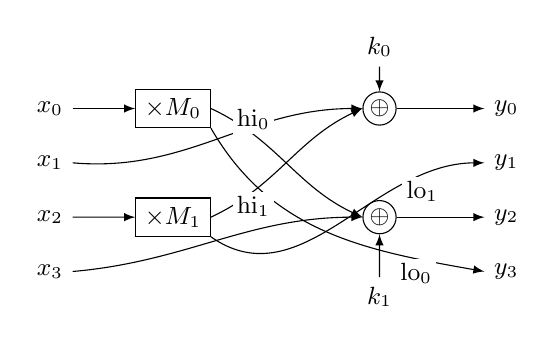
\begin{tikzpicture}[>=latex, scale=0.92, every node/.style={font=\small}]
	\node (x0) at (0, 0)    {$x_0$};
	\node (x1) at (0,-0.75) {$x_1$};
	\node (x2) at (0,-1.5)  {$x_2$};
	\node (x3) at (0,-2.25) {$x_3$};
	\node[draw]  (M0) at (1.7, 0)    {\texttt{$\times M_0$}};
	\node[draw]  (M1) at (1.7,-1.5)  {\texttt{$\times M_1$}};
	\node[draw, circle, inner sep=0.9pt] (c0) at (4.55, 0)    {$\oplus$};
	\node[draw, circle, inner sep=0.9pt] (c1) at (4.55,-1.5)  {$\oplus$};
	\node (y0) at (6.3, 0)    {$y_0$};
	\node (y1) at (6.3,-0.75) {$y_1$};
	\node (y2) at (6.3,-1.5)  {$y_2$};
	\node (y3) at (6.3,-2.25) {$y_3$};
	\node (k0n) at (4.55, 0.85)  {$k_0$};
	\node (k1n) at (4.55,-2.6)   {$k_1$};
	\draw[->] (x0) -- (M0);
	\draw[->] (x2) -- (M1);
	\draw[->] (x1.east) to[out=-5,in=180] (c0.west);
	\draw[->] (x3.east) to[out=5,in=180] (c1.west);
	\draw[->] (M0.east) to[out=-25,in=155] node[pos=0.25, above, fill=white, inner sep=1.5pt]{$\mathrm{hi}_0$} (c1.west);
	\draw[->] (M0.south east) to[out=-60,in=170] node[pos=0.8, below, fill=white, inner sep=1.5pt]{$\mathrm{lo}_0$} (y3.west);
	\draw[->] (M1.east) to[out=25,in=205] node[pos=0.25, below, fill=white, inner sep=1.5pt]{$\mathrm{hi}_1$} (c0.west);
	\draw[->] (M1.south east) to[out=-35,in=180] node[pos=0.8, below, fill=white, inner sep=1.5pt]{$\mathrm{lo}_1$} (y1.west);
	\draw[->] (k0n) -- (c0.north);
	\draw[->] (k1n) -- (c1.south);
	\draw[->] (c0.east) -- (y0.west);
	\draw[->] (c1.east) -- (y2.west);
\end{tikzpicture}
\end{center}

\begin{align*}
(y_0,\, y_1,\, y_2,\, y_3) &= (\mathrm{hi}_1 \oplus x_1 \oplus k_0,\; \mathrm{lo}_1,\; \mathrm{hi}_0 \oplus x_3 \oplus k_1,\; \mathrm{lo}_0),
\end{align*}
where $(\mathrm{hi}_j, \mathrm{lo}_j)$ are the high/low 32-bit halves of $M_j x_{2j}$.

\end{frame}

\begin{frame}
\frametitle{Philox: the key schedule (Weyl sequence)}

Each round must use {\blue different subkeys}, otherwise round symmetry would leak
structure. Between two rounds, the subkeys advance by a fixed {\blue Weyl step}:
\[
(k_0,\, k_1) \;+\!\!=\; (W_0,\, W_1)
\]
with the constants
\[
W_0 = \mathtt{9E3779B9}_{16}, \qquad W_1 = \mathtt{BB67AE85}_{16},
\]
taken as odd parts of well-chosen irrationals ($W_0$ from the golden ratio
$\varphi$, $W_1$ from $\sqrt{3}-1$).

\begin{itemize}
\item
A single 64-bit integer addition per round: {\blue cheap}.
\item
The schedule is invertible, so each round stays a bijection.
\end{itemize}

\end{frame}

\begin{frame}
\frametitle{Philox: from blocks to a number sequence}

After $r = 10$ rounds, the counter/key pair has been fully scrambled into a block
$R = E_K(C)$. We map a 32-bit word to $[0,1)$ with a plain division:
\[
u = \frac{R_j}{2^{32}} \in [0,1),
\]
so each call provides up to $4$ uniforms (or a 128-bit block).

\vfill

Summary of the {\blue streaming model}:
\begin{itemize}
\item
draw next block: increment the counter, $C \leftarrow C + 1$;
\item
jump $m$ blocks ahead: $C \leftarrow C + m$ (an integer addition);
\item
switch stream: change the key $K$;
\item
no state to store or synchronize: natural for GPUs and parallel workers.
\end{itemize}

\end{frame}

\begin{frame}
\frametitle{Jump ahead}

\begin{itemize}
	\item 
A very useful possibility proposed by some implementation is the possibility to make a jump of $m$ positions in the random number sequences, with $m$ very large.
\item
This allows one to easily define independent random variables.
\item
Useful in simulation when relying on common random numbers.
\end{itemize}

Historically, MRG32k3a was one of the few generators offering built-in functions for independent streams and substreams. Today, the library \texttt{RandomDataStreams.jl} extends this capability to a wide variety of generators in a unified framework.

\end{frame}

	\begin{frame}
	\frametitle{Streams and Substreams}

	\begin{center}
	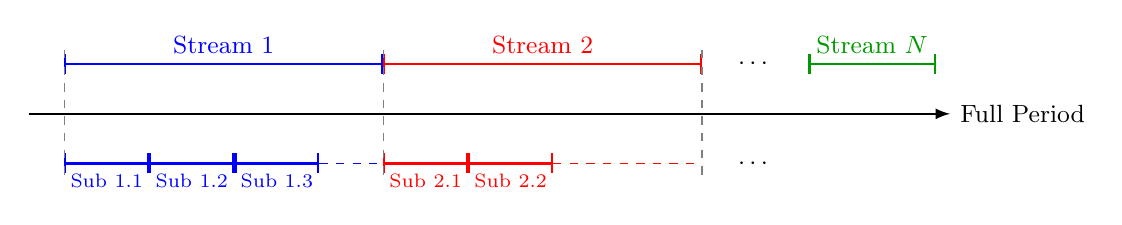
\begin{tikzpicture}[>=latex, scale=0.9, font=\small]
		% Main backbone
		\draw[thick, ->] (0, 0) -- (13, 0) node[right] {Full Period};
		
		% Stream 1
		\draw[blue, thick, |-|] (0.5, 0.7) -- (5.0, 0.7) node[midway, above] {Stream 1};
		\draw[blue, thick, |-|] (0.5, -0.7) -- (1.7, -0.7) node[midway, below, font=\scriptsize] {Sub 1.1};
		\draw[blue, thick, |-|] (1.7, -0.7) -- (2.9, -0.7) node[midway, below, font=\scriptsize] {Sub 1.2};
		\draw[blue, thick, |-|] (2.9, -0.7) -- (4.1, -0.7) node[midway, below, font=\scriptsize] {Sub 1.3};
		\draw[blue, dashed] (4.1, -0.7) -- (5.0, -0.7);

		% Stream 2
		\draw[red, thick, |-|] (5.0, 0.7) -- (9.5, 0.7) node[midway, above] {Stream 2};
		\draw[red, thick, |-|] (5.0, -0.7) -- (6.2, -0.7) node[midway, below, font=\scriptsize] {Sub 2.1};
		\draw[red, thick, |-|] (6.2, -0.7) -- (7.4, -0.7) node[midway, below, font=\scriptsize] {Sub 2.2};
		\draw[red, dashed] (7.4, -0.7) -- (9.5, -0.7);
		
		% Stream k
		\node at (10.25, 0.7) {$\cdots$};
		\node at (10.25, -0.7) {$\cdots$};
		
		\draw[green!60!black, thick, |-|] (11.0, 0.7) -- (12.8, 0.7) node[midway, above] {Stream $N$};
		
		% Vertical guides
		\draw[dashed, gray] (0.5, 0.9) -- (0.5, -0.9);
		\draw[dashed, gray] (5.0, 0.9) -- (5.0, -0.9);
		\draw[dashed, gray] (9.5, 0.9) -- (9.5, -0.9);
	\end{tikzpicture}
	\end{center}

	\begin{itemize}
	\item {\blue Streams:} The global sequence is partitioned into huge, non-overlapping segments (e.g., $2^{127}$ values).
	\item {\blue Substreams:} Each stream is further subdivided (e.g., $2^{76}$ values).
	\item \textbf{Use case:} Allocate one stream per scenario, and advance to the next substream for each simulation run (replication) to maintain alignment (Common Random Numbers).
	\end{itemize}

	\end{frame}

	\begin{frame}[fragile]
	\frametitle{RandomDataStreams.jl}

	A Julia package providing a unified framework for independent streams and substreams.
	
	\vspace{0.2cm}
	\textbf{Installation:} \texttt{] add RandomDataStreams}

	\vspace{0.4cm}
	{\blue Code example:} One stream per scenario, one substream per replication.
	
	\begin{footnotesize}
	\begin{semiverbatim}
using RandomDataStreams

gen = MRG32k3aGen()     # Generator instance
rng = next_stream!(gen) # Independent stream (Scenario 1)

# Replication 1
u1 = rand(rng)

# Replication 2
next_substream!(rng)    # Fast jump to the next substream
u2 = rand(rng)
	\end{semiverbatim}
	\end{footnotesize}

	\end{frame}

	\begin{frame}
		\frametitle{Non-uniform random variables generation}
		\label{chap:nonuniform}
		
		A good reference: Luc Devroye, \textsl{Non-Uniform
			Random Variate Generation},
		\url{http://luc.devroye.org/rnbookindex.html}.
		
		\mbox{}
		
		Assume that we have a good uniform random variates generator, but we
		want to generate random variables following various probability laws:
		Normal, Weibull, Poisson, binomial,\ldots
		
		\mbox{}
		
		The desired properties are:
		\begin{itemize}
			\item
			correct method (or good approximation);
			\item
			as simple as possible, but as fast as possible;
			\item
			low memory consumption;
			\item
			robust;
			\item
			compatible with variance reduction technique (as quasi-Monte Carlo).
		\end{itemize}
		
	\end{frame}
	
	\begin{frame}
		\frametitle{Inversion Method: Principle}

		Consider a random variable $X$ with cumulative distribution function $F$.
		Let $U \sim U (0, 1)$ and define:
		\[
		X = F^{-1}(U) = \min \lbrace x : F (x)  \geq U \rbrace \quad \textrm{\textcolor{red}{(Generalized inverse)}}.
		\]
		Then,
		\[
		P [X \leq x] = P [F^{-1}(U) \leq x] = P [U \leq F (x)] = F (x),
		\]
		i.e., $X$ precisely follows the desired distribution.
		
		\vspace{0.4cm}
		This foundational principle applies universally:
		\begin{itemize}
			\item \textbf{Continuous case:} $F(X) \sim U[0,1]$;
			\item \textbf{Discrete case:} ensures $P[X = x_i] = p(x_i)$ assuming ordered $x_i$;
			\item \textbf{Mixed distributions:} works seamlessly.
		\end{itemize}
	\end{frame}
	
	\begin{frame}
		\frametitle{Inversion: The Gold Standard}

		\begin{itemize}
		    \item \textbf{Monotonic mapping:} Inversion guarantees a monotonic relationship between the uniform draw $U$ and the generated variable $X$.
		    \vspace{0.3cm}
		    \item \textbf{Variance Reduction:} This monotonicity is strictly required by variance reduction techniques like \textit{Common Random Numbers} (CRN) or \textit{Antithetic Variates}, which break down with other generation methods (like acceptance-rejection).
		    \vspace{0.3cm}
		    \item \textbf{Copulae:} It is the preferred method when building dependent joint distributions using copulae.
		\end{itemize}

	\end{frame}
	
	\begin{frame}
		\frametitle{Inversion (2)}
		
		\begin{itemize}
			\item
			{\red Advantage}: monotone, only one $U$ for all $X$.
			\item
			{\red Weakness}: for some laws, $F$ is very difficult to invert.
			But we can often approximate $F^{-1}$.
		\end{itemize}
		
		\mbox{}
		
		{\red Example}: normal law.\\
		If $Z \sim N (0, 1)$, then $X =  \sigma Z + \mu \sim N (\mu, \sigma^2)$.
		
		It is therefore sufficient to be able to generate a $N (0, 1)$, of
		density $f (x) = (2 \pi)^{-1/2} e^{-x^2 /2}$.
		
		We do not have any formula for $F (x)$ or $F^{-1}(x)$.
		Efficient codes however exist to approximate $F^{-1}(x)$.
		
		\mbox{}
		
		Chi-square, gamma, beta, etc.: it is much more complicated since the
		form of $F^{-1}$ depends on the distribution parameters.
		
	\end{frame}
	
	\begin{frame}
		\frametitle{Inversion for discrete distributions}
		
		Recall that
		\begin{align*}
			p(x_i) = P [X = x_i];\quad 
			F (x) = \sum_{x_i \leq x} p(x_i).
		\end{align*}
		
		We have to generate $U \sim U(0,1)$, search 
		\[
		I = \min \lbrace i \mid F (x_i)  \geq U \rbrace
		\]
		and return $X = x_I$.
		
		\vspace{0.4cm}
		{\red Initialization}: store the values $x_i$ and the cumulative probabilities $F (x_i)$ in arrays, for $i = 1, \ldots, n$.
		
		\vspace{0.2cm}
		Various algorithms can perform this search. Their efficiency heavily depends on the distribution and the number of outcomes $n$.
	\end{frame}
	
	\begin{frame}
		\frametitle{Discrete Inversion: Search Algorithms}
		
		\begin{enumerate}
			\item \textbf{\blue Linear search} (time in $\mathcal{O}(n)$): \\
			\texttt{generate} $U \sim U (0, 1)$; \\
			$i \leftarrow 1$; \\
			\texttt{while} $F (x_i) < U$ \texttt{do} $i \leftarrow i + 1$; \\
			\texttt{return} $x_i$.

			\vspace{0.5cm}
			
			\item \textbf{\blue Binary search} (time in $\mathcal{O}(\log(n))$): \\
			\texttt{generate} $U \sim U (0, 1)$; \\
			$L \leftarrow 0$; $R \leftarrow n$; \\
			\texttt{while} $L < R - 1$ \texttt{do} \\
			\quad $m \leftarrow \lfloor (L + R)/2 \rfloor$; \\
			\quad \texttt{if} $F (x_m) < U$ \texttt{then} $L \leftarrow m$ \texttt{else} $R \leftarrow m$; \\
			\texttt{return} $x_R$.
		\end{enumerate}
		
	\end{frame}
	
	\begin{frame}
		\frametitle{Other approaches: composition}
		
		Assume that $F$ is a convex combination of several cumulative
		distribution functions:
		\[
		F (x) = \sum_{j = 1}^{\infty} p_j F_j (x),
		\]
		and that it is easier to invert each $F_j$, $j = 1, 2, \ldots$, than $F$.
		
		\mbox{}
		
		Generate $J = j$ with the probability $p_j$, then generate $X$
		following $F_J$.
		
		\mbox{}
		
		The method therefore requires two uniforms for each random variable,
		and exploits the decomposition
		\[
		P[ X \leq x ] = \sum_{j = 1}^{\infty} P[ X \leq x | J = j] P[J = j] = \sum_{j = 1}^{\infty} F_j(x)p_j.
		\]
		
	\end{frame}
	
	\begin{frame}
		\frametitle{Convolution}
		
		{\red Convolution}. Assume that
		\[
		X = Y_1 + Y_2 + \ldots + Y_n,
		\]
		where the $Y_i$ are independent, of given laws.
		We generate the $Y_i$, $i = 1,\ldots,n$, and we sum.
		
		\mbox{}
		
		Examples: Erlang (sum of exponentials with same mean), binomial.
		
		\mbox{}
		
		\mbox{}
		
		{\red Acceptance/rejection}: the most important technique after inversion.
		
		\mbox{}
		
		We consider the case where $X$ is continuous (the discrete case is
		analogous).
		Let $f(x)$ be the density of $X$, and let $t$ be a ``hat'' function that
		dominates $f$, i.e. $f (x) \leq t(x)\ \forall\, x$.
		
	\end{frame}
	
	\begin{frame}
		\frametitle{Acceptance/rejection}
		
		We can normalize $t$ in a density $r$:
		\[
		r(x) = t(x)/a,\mbox{ where }a = \int_{-\infty}^{\infty} t(s)ds.
		\]
		We choose $t$ so that
		\begin{enumerate}
			\item
			it is easy to generate random variables of density $r$;
			\item
			$a$ is small (close to 1), or in other terms, $t(x)$ is close to $f(x)$.
		\end{enumerate}
		The choice of $t$ may be automatized.
		
		\mbox{}
		
		\begin{minipage}{0.52\linewidth}
			{\blue Algorithm}: Repeat
			\begin{enumerate}
				\item
				generate $Y$ of density $r(x)$;
				\item
				generate $U \sim U (0, 1)$ independently of $Y$;
				\item
				until $U \leq f (Y )/t(Y )$;
				\item
				return Y.
			\end{enumerate}
		\end{minipage}
		\begin{minipage}{0.47\linewidth}
			
\includegraphics[width=0.7\linewidth]{NormalRejectGrid.eps}
		\end{minipage}
		
	\end{frame}
	
	\begin{frame}
		\frametitle{Particular cases}
		
		Sometimes, we can benefit from mathematical transformations.\\
		The main weakness is that they are seldom compatible with variance
		reduction techniques.
		
		\mbox{}
		
		{\blue Example}: Box-Muller method for the normal law.
		
		\mbox{}
		
		{\red Idea}: it is easier to generate a point $(X, Y)$ from the bivariate
		normal law, of density on $\rit^2$
		\[
		f (x, y ) = \frac{1}{2\pi} e^{-(x^2 +y^2 )/2}.
		\]
		We change the cartesian coordinates $(X,Y)$ by the polar coordinates $(R, \Theta)$:\\
		\[
		R^2 = X^2 + Y^2, \quad X = R \cos \Theta, \quad Y = R \sin \Theta.
		\]
		
		It gives an elegant approach, but incompatible with variance reduction techniques and can be slower than inversion.
		
\end{frame}

\begin{frame}
\frametitle{Box-Muller Algorithm}

\begin{enumerate}
\item
Independently draw $U_1$, $U_2$ from a $U(0,1)$ distribution.
\item
Set
\begin{align*}
R &= \sqrt{-2 \log (U_1)} \\
\theta &= 2 \pi U_2
\end{align*}
\item
Set
\begin{align*}
X &= R \cos(\theta) \\
Y &= R \sin(\theta)
\end{align*}
\end{enumerate}
		
\end{frame}

\begin{frame}
\frametitle{Multivariate distributions}

What if we want to draw from $\bsX: \Omega \rightarrow \calX \subseteq \RR^d$?

General approach:
\begin{itemize}
	\item Generate the marginals
	\item Combine the marginals as desired.
\end{itemize}
		
\end{frame}

\begin{frame}
\frametitle{Multivariate distributions: simple cases}

\begin{itemize}
\item 
Ideally, we can explicitly transform the marginals.
\item
Example: multivariate normal $\bsX \sim \calN(\bsmu, \Sigma)$, with
$$
\bsmu =
\begin{pmatrix}
	\mu_1 \\ \mu_2 \\ \vdots \\ \mu_d
\end{pmatrix}
\qquad
\Sigma = 
\begin{pmatrix}
	\sigma^2_1 & \sigma_{1,2} & \ldots & \sigma_{1,d} \\
	\sigma_{1,2} & \sigma^2_2 & \ldots & \sigma_{2,d} \\
	\vdots & \vdots & \ddots & \vdots \\
	\sigma_{1,d} & \sigma_{2,d} & \ldots & \sigma^2_d 
\end{pmatrix}
$$
Then,
$$
\bsX = \bsmu + L\bsZ, \quad \text{where } \bsZ \sim \calN(\bszero, \bsI)
$$
with $\Sigma = LL^T$, and $L$ is the Cholesky factor.

Drawing from $\calN(\bszero,\bsI)$: generate $d$ $\calN(0,1)$ independently.
\end{itemize}
		
\end{frame}

\begin{frame}
\frametitle{Multivariate distributions: copulae}

\textbf{Intuition:} Copulae allow us to completely decouple the \textit{marginal distributions} (what each variable looks like individually) from their \textit{dependence structure} (how they move together).

\mbox{}

A $d$-variate \textcolor{red}{copula} $C: [0, 1]^d \rightarrow [0, 1]$ is the cdf of a random vector
$(U_1,\ldots, U_d)$ with $U(0, 1)$ margins:
$$
C(u) = P[U_1 \leq u_1,\ldots, U_d \leq u_d]
$$
where
$$
P[U_j \leq u_j] = u_j
$$
for $j = 1,\ldots,d$, and $0 \leq u_j \leq 1$.

\end{frame}

\begin{frame}
\frametitle{Sklar's theorem}

\begin{theorem}[Sklar's theorem (1959)]
	\begin{itemize}
		\item 
	Let $H$ be a multivariate distribution function with margins $F_1,\ldots, F_d$.
	There exists a copula $C$ such that
$$
		H(x_1, \ldots, x_d) = C \left( F_1(x_1), \ldots, F_d(x_d) \right), \quad x_1, \ldots, x_d \in \overline{\RR}.
%		\label{eq:Copulas}
$$
	If $F_i$, $i = 1, \ldots, d$, are continuous then $C$ is unique. Otherwise $C$ is uniquely determined on the Cartesian product of the range of the marginals $F_1 \left( \overline{\RR} \right) \times \ldots \times F_d \left( \overline{\RR} \right)$.
	\item
	Conversely, if $C$ is a copula and $F_1, \ldots, F_d$ are univariate distribution functions, then the function $H$ defined above is a multivariate distribution function with margins $F_1, \ldots, F_d$.
	\end{itemize}
\end{theorem}

\end{frame}

\begin{frame}
\frametitle{Copula}

If we know the joint CDF $F$ and the marginals $F_1,\ldots,F_d$, we can find the copula via
$$
C(u_1,\ldots,u_d) = F\left(F_1^{-1}(u_1),\ldots,F_d^{-1}(u_d)\right),
$$
where $F_j^{-1}(\cdot)$ is the generalized inverse for margin $j$:
$$
F_j^{-1}(u) = \min \{ x \,:\, F_j(x) \geq u \}.
$$

\end{frame}

\begin{frame}
\frametitle{Fréchet–Hoeffding bounds}

Any bivariate copula $C$ verifies
$$
\max(u + v - 1, 0) \leq C(u, v) \leq \min(u, v), \quad (u,v) \in [0,1]^2,
$$
equivalently, for the joint cdf $H(x,y) = C(F_X(x), F_Y(y))$,
$$
\max(F_X(x) + F_Y(y) - 1, 0) \leq H(x, y) \leq \min(F_X(x), F_Y(y)).
$$

\mbox{}

\textcolor{blue}{Upper bound proof}
	\begin{align*}
		H(x, y) &= P[X \leq x \cap Y \leq y] \\
		&\leq \min\left(P[X \leq x], P[Y \leq y]\right) = \min(F_X(x), F_Y(y))
	\end{align*}
	since $\lbrace X \leq x \rbrace \cap \lbrace Y \leq y \rbrace \subseteq \lbrace X \leq x \rbrace$ and $\subseteq \lbrace Y \leq y \rbrace$.

\end{frame}

\begin{frame}
\frametitle{Fréchet–Hoeffding bounds}

\textcolor{blue}{Lower bound proof}
\begin{align*}
1 - H(x,y) &= P[X > x \cup Y > y] \\
& \leq P[X > x] + P[Y > y] \\
& = 1 - F_X(x) + 1 - F_Y(y)
\end{align*}
Thus,
$$
H(x,y) \geq F_X(x) + F_Y(y) - 1.
$$

\mbox{}

\textcolor{red}{Note:} this can be viewed as a particular case of the Bonferroni inequality
$$
P \left[ \cap_{i = 1}^d A_i \right] \geq 1-d+\sum_{i = 1}^d P [A_i].
$$

\end{frame}

\begin{frame}
\frametitle{Gaussian copula}

$$
	C \left( F_1(x_1), \ldots, F_d(x_d) \right)
	= \Phi_{\Sigma} \left( \Phi^{-1} \left( F_1(x_1) \right),\ldots, \Phi^{-1}\left( F_d(x_d) \right) \right),
$$
where
\begin{itemize}
	\item $\Phi$ is the cdf of a $\calN(0,1)$,
	\item $\Phi_{\Sigma}$ is the cdf of a $d$-dimensional $\calN(\bszero,\Sigma)$.
\end{itemize}

\end{frame}

\begin{frame}
\frametitle{Copulae estimation}

\begin{itemize}
	\item Parametric estimation;
	\item Non-parametric estimation;
	\item Machine-learning models (see Jutras-Dubé et al., \textit{Transportation Research Part C}, 2024).
\end{itemize}

\end{frame}

\begin{frame}
\frametitle{Further reading}

\begin{itemize}
    \item \textbf{General RNG principles:} L'Ecuyer, P. (2012). \textit{Random Number Generation}. \url{https://www.iro.umontreal.ca/~lecuyer/myftp/papers/wsc12rng.pdf}
    \item \textbf{Philox \& CBRNGs:} Salmon et al. (2011). \textit{Parallel Random Numbers: As Easy as 1, 2, 3}. \url{https://doi.org/10.1145/2063384.2063405}
    \item \textbf{PCG family:} O'Neill, M. E. (2014). \url{https://www.pcg-random.org/}
    \item \textbf{xoshiro / xorshift:} Blackman, D. \& Vigna, S. (2021). \textit{Scrambled Linear Pseudorandom Number Generators}. \url{https://prng.di.unimi.it/}
    \item \textbf{Non-uniform generation:} Devroye, L. (1986). \textit{Non-Uniform Random Variate Generation}. \url{http://luc.devroye.org/rnbookindex.html}
\end{itemize}

\end{frame}

\end{document}